% 下面这种字体警告可以不理会
% Font "STFangsong" does not contain requested Script (fontspec) "CJK".

% LTeX: language=zh-CN
\documentclass[a4paper,oneside,UTF8]{ctexart} %A4纸,单面,UTF-8

\usepackage{geometry}
\geometry{left=3.5cm,right=2.5cm,top=2.54cm,bottom=2.54cm}
                                            % 支持版面尺寸设置
\renewcommand{\baselinestretch}{1.55}       % 设置行距
\renewcommand{\CJKglue}{\hskip -0.1 pt plus 0.08\baselineskip}
\ziju{0.1}                                 % 控制字间距,使每行 33 个汉字

\usepackage{fontspec}                    %设置字体需要的宏包
\setmainfont{Times New Roman}           %设置西文字体为Times New Roman
\renewcommand{\normalsize}{\zihao{-4}}  %设置正文字号为小四

\setcounter{secnumdepth}{5}                                                                                     %
\ctexset { section = { name={第,章},number={\chinese{section}},format={\centering \heiti \zihao {3}} } }         %
\ctexset { subsection = { name={$\S${ },},format={\heiti \zihao {4}} } } %设置各级系统的编号格式
\ctexset { subsubsection = { name={$\S${ },},format={\heiti \zihao {-4}} } }          %
\ctexset { paragraph = { name={,},number={\chinese{paragraph}},format={\songti \zihao {-4}} } }               %
\ctexset { subparagraph = { name={,},number={\arabic{subparagraph}},format={\songti \zihao {-4}} } }           %

% Include other packages here, before hyperref.
\usepackage{graphicx}

\usepackage{amsmath}
\usepackage{amsthm}
\usepackage{amssymb}

\usepackage{longtable}
\usepackage{tabularx}
\usepackage{booktabs}
\usepackage{multirow}

\usepackage{caption}
\usepackage{subcaption}
\usepackage{pdflscape}
\usepackage{float}
\usepackage[bottom]{footmisc}

\usepackage[dvipsnames]{xcolor}
\usepackage[breaklinks,colorlinks]{hyperref}
\usepackage[backend=biber,style=gb7714-2015]{biblatex}

% 自己定义需要的环境
\newtheorem{theorem}{定理}[section]
\newtheorem{definition}{定义}[section]
% 引用时需要根据具体类型使用具体的引用命令
\newcommand{\thmref}[1]{定理~\ref{#1}}
\newcommand{\lemref}[1]{引理~\ref{#1}}
\newcommand{\propref}[1]{命题~\ref{#1}}
\newcommand{\corref}[1]{推论~\ref{#1}}
\newcommand{\defref}[1]{定义~\ref{#1}}
\newcommand{\eqnref}[1]{(\ref{#1})}

% 仅针对下面这几类,也可以都使用/autoref命令
\renewcommand{\theoremautorefname}{\text{定理~}}
\renewcommand{\figureautorefname}{\text{图~}}
\renewcommand{\tableautorefname}{\text{表~}}
\renewcommand{\figurename}{\kaishu\zihao{5}图}
\renewcommand{\tablename}{\kaishu\zihao{5}表}

\graphicspath{ {./images/} }
\addbibresource{ref.bib}

\begin{document}

\title{河南科技大学数学学院论文翻译任务模版}

\author{Xuyou Mo\footnote{这是一个带注释的标记。} \quad Cunzai Bu\footnote{这是一个带注释的标记。} \quad Youren Mei \\
School of Mathematics, Daxue University \\
Chengshi, Shengfen 123456, China \\
{\tt\small test1email@123.com \quad test2email@321.com \quad test3email@abc.com}
% For a paper whose authors are all at the same institution,
% omit the following lines up until the closing ``}''.
% Additional authors and addresses can be added with ``\and'',
% just like the second author.
% To save space, use either the email address or home page, not both
\and
Second Author\\
Institution2\\
First line of institution2 address\\
{\tt\small secondauthor@i2.org}
}
\date{}
\maketitle

\noindent \textbf{摘要:} 这里是摘要

\noindent \textbf{关键字:} 这里是关键字

\section{测试表格}

测试引用表格\autoref{tab:example}

\begin{table}[htbp]
    \centering
    \begin{tabular}{@{}lc@{}}
        \toprule
        Method & Frobnability           \\
        \midrule
        Theirs & Frumpy                 \\
        Yours  & Frobbly                \\
        Ours   & Makes one's heart Frob \\
        \bottomrule
    \end{tabular}
    \caption{\kaishu\zihao{5}测试表格}
    \label{tab:example}
\end{table}

\section{测试图片}

测试引用图片\autoref{fig:testimage}
\begin{figure}
    \centering
    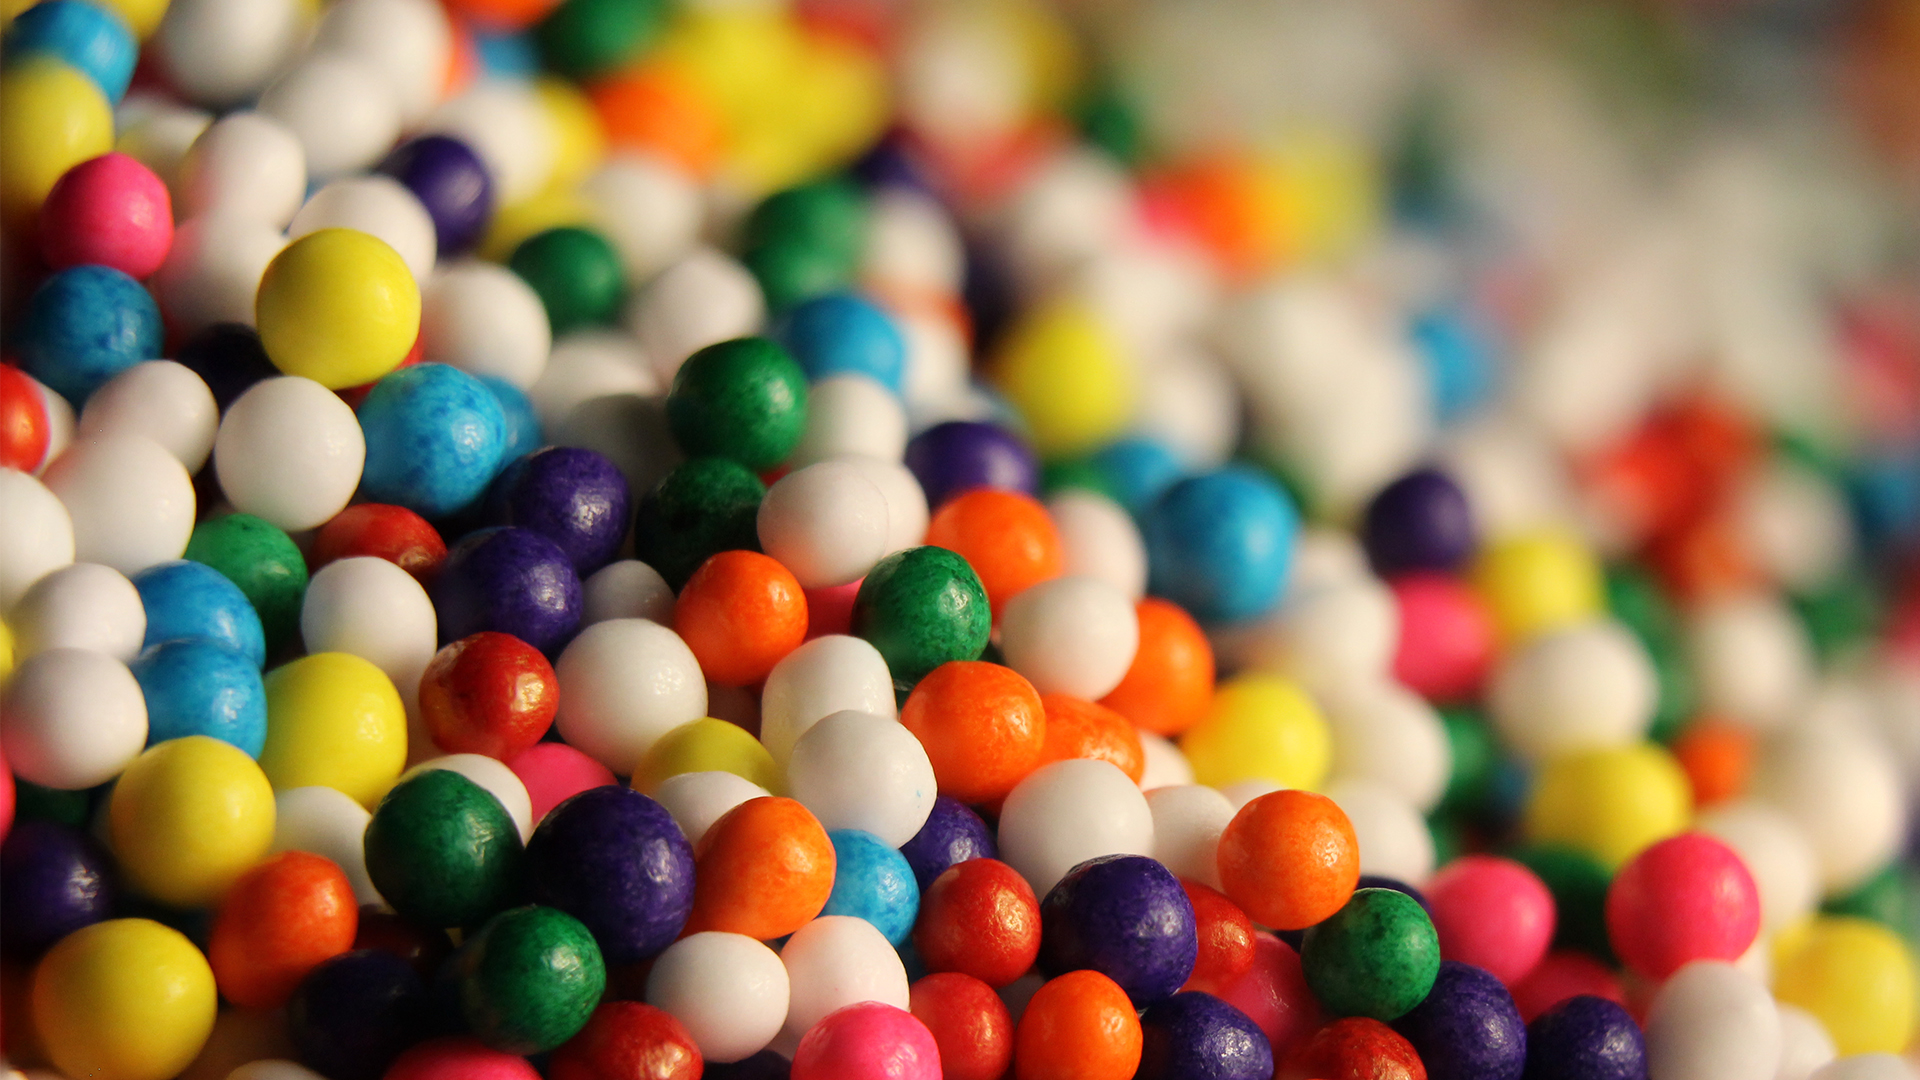
\includegraphics[width=1.0\linewidth]{figure_example1.jpg}
    \caption{\kaishu\zihao{5}测试图片}
    \label{fig:testimage}
\end{figure}

\section{测试公式}
测试公式
$$
\begin{aligned}
    \nabla \cdot \boldsymbol{E}=\frac{\rho}{\varepsilon_0}
\end{aligned}
$$

\begin{theorem}
    这里是一个定理
    $$
    1 + 1 = 3
    $$
    \label{thm:113}
\end{theorem}

测试引用定理\autoref{thm:113}
\section{测试引用}

这里测试引用\cite{dai2022explicit}

\printbibliography

\end{document}
